
%\new{
%The cost of performing a calculation of the nucleon axial form factor,
% both in terms of computation time and human time for analysis,
% is significantly more than what is required for a computation the axial charge.
%Despite the active efforts collaborations have had in computing the axial form factor,
% the costs have been a limiting factor in the availability of results.
%}

The main deliverables from LQCD calculations of the axial form factor
 are the axial and induced pseudoscalar form factors taken in the continuum-chiral
 and infinite volume limits, complete with a set of parameterization coefficients
 and covariance matrix.
Though the axial charge and radius are useful for connecting with low-energy applications,
 such as pion electroproduction and neutron decay,
 the needs of neutrino physics in the few-GeV energy range depend
 on the full momentum transfer dependence of the form factor.
 This is especially true considering the agreement between LQCD and experiment
 for the axial radius taken together with the observation that
 LQCD prefers a slower form factor fall off than experiment,
 as shown in Figure~\ref{fig:gaq2_overlay}.
If the axial radius were the only parameter determining the form factor $Q^2$ dependence,
 then these two observations are incompatible.
Though the form factor shape, especially when allowed to explore its full uncertainty,
 is decidedly \emph{not} a dipole, the central value curve determined
 from experiment appears to be dipole-like.
Restricting to dipole shape only, agreement with the axial radius at $Q^2=0$
 would mean the axial form factor should agree over the entire relevant $Q^2$ range,
 a statement that is not supported by the LQCD data.
There is no reason to expect nature to prefer a dipole-like parameterization ---
 the experimental preference toward a dipole-like parameterization is based on
 a few datasets from the 1970's and 1980's~\cite{ANL_Barish_1977, BNL_Baker_1981, Kitagaki:1983px}
 with $O(10^3)$ events at most,
 on deuterium targets with nuclear corrections that are likely underestimated~\cite{Meyer:2016oeg}.
In addition, the dipole parameterization violates
 unitarity constraints imposed by QCD~\cite{Bhattacharya:2011ah},
 %and is primarily motivated by its asymptotic behavior at high-$Q^2$,
 %a regime well outside of the kinematic range probed by neutrino scattering experiments.
 and although it has the expected asymptotic behavior at high-$Q^2$,
 this occurs for a regime well outside of the kinematic range probed
 by neutrino scattering experiments.

% \done{I don't think the use of the dipole for FA was motivated by its asymptotic behaviour? I thought they just tried out a few FFs and found the dipole worked best, but didn't really have a strong theory motivation for any of theose they tried.}
% \asm{You're right: as written, the statement is/was wrong.
% I think dipole is also, in some rough sense,
% the fourier transform of an exponential decay wavefunction profile.
% My thought process was that people cling to dipole by saying it has the
%  correct asymptotic behavior (unlike e.g. monopole, which was also tried),
%  but that the preference is unfounded because it only occurs well outside
%  of the region of interest.
% Updated to reflect these thoughts better.
% }


Figure~\ref{fig:gaq2_overlay} shows the status of existing calculations of
 the nucleon axial form factor from LQCD,
 compared to the axial form factor obtained from neutrino scattering
 with deuterium in Ref.~\cite{Meyer:2016oeg}.
The RQCD~\cite{RQCD:2019jai} and NME~\cite{Park:2021ypf} collaborations
 have the most mature analyses with several ensembles that probe a range of
 systematic effects.
These computations each have their own methods for addressing the
 excited state contaminations discussed in Section~\ref{sec:lqcd_pcac},
 which successfully restore the GGT relation.
RQCD modify the parameterization used to fit the correlation function
 to better constrain the expected shape of excited state contamination from the $N\pi$ states \new{based upon expectations from $\chi$PT~\cite{Bar:2018xyi}.}
NME test a variety of Bayesian fits to constrain the excited state contributions,
 where their preferred fit enforces a tight prior on the nucleon-pion state
 at the energy expected from a naive dispersion relation.
\new{It should be noted that expectations from $\chi$PT suggest that the dominant excited state contamination of nucleon matrix element of $A_4$ is from a single $N\pi$ state, while for $A_3$, it is a tower of $N(\mathbf{p})\pi(-\mathbf{p})$ states with all relative momentum, which is likely not well described by a single $N\pi$ state.}
Because these two results are based on several ensembles,
 their fits are parameterized and plotted as bands rather than as scatter points
 to distinguish them from estimates on single ensembles.

\begin{figure}[hbt!]
\centering
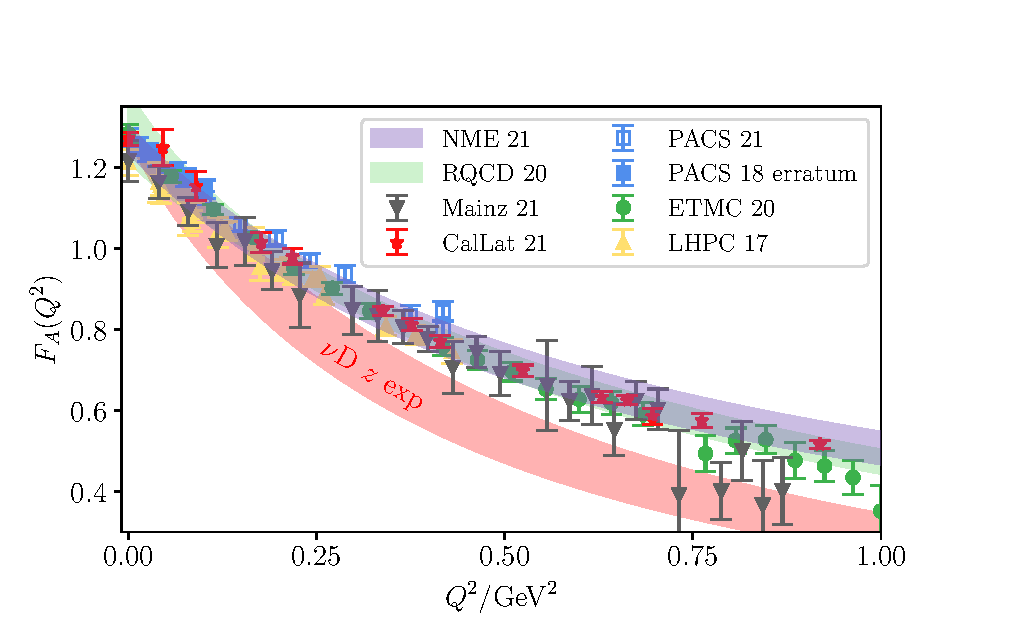
\includegraphics[width=0.75\textwidth]{plots/gaq2-overlay-standalone.pdf}
\vspace{10pt}
\caption{
Published results for the axial form factor obtained from LQCD,
 compared with the deuterium extraction from Ref.~\cite{Meyer:2016oeg}.
Results taken from only a single ensemble are plotted as scatter points.
These single-ensemble results will have small but unknown corrections due to chiral, continuum,
 and finite volume systematic shifts.
The NME~\cite{Park:2021ypf} and RQCD~\cite{RQCD:2019jai}
 results are both obtained from fits to several ensembles.
The RQCD perform the full chiral-continuum and finite volume extrapolations to the data,
 fitting to each of the form factors independently for each ensemble but providing
 the constraint that the form factors must satisfy the GGT relation in the continuum.
The NME collaboration also performed a chiral-continuum and finite volume extrapolation
 on their data, but found significantly larger uncertainties
The plotted NME result is obtained from a fit to their five largest volume ensembles neglecting
 effects from lattice spacing, finite volume, and pion mass.
As a rough estimate, the NME publication~\cite{Park:2021ypf} states that
 the uncertainties are about a factor of 5 larger if the fits are relaxed
 to allow for pion mass or lattice spacing effects.}
% \cw{Why are there two PACS 21 datapoints on top of each other at ~0.4 GeV$^2$}}
% \asm{Two different ways of constructing momentum vectors of magnitude 3: (2,2,1) and (3,0,0)}
\label{fig:gaq2_overlay}
\end{figure}

The ETMC~\cite{Alexandrou:2020okk}, LHPC~\cite{Hasan:2017wwt},
 PACS~\cite{Ishikawa:2018rew,Shintani:2018ozy,Ishikawa:2021eut}, and CalLat~\cite{Meyer:2021vfq}
 results have just a few ensembles, so scatter points obtained from fitting
 are shown rather than the form factor parameterization to distinguish
 them from extrapolated results.
Though these results are expected to be close to the physical point results,
 they will have unquantified systematic shifts.
The ETMC has three ensembles, two of which have only 2 flavors of sea quarks
 and will be subject to systematics from neglecting sea effects from strange quarks.
%\done{Should it be entirely obvious to a non-expert reader why you've written 2+1+1 rather than 4? (asking for a friend)}
%\asm{No. Not described in LQCD intro section as far as I see, so jargon removed.}
The form factor data from the remaining ETMC ensemble,
 a physical pion mass ensemble with 4 flavors of sea quarks \new{(up, down, strange and charm)},
 is shown in Fig.~\ref{fig:gaq2_overlay}.
The PACS results are on two different ensembles with physical pion mass,
 with volumes of $(5.5~{\rm fm})^3$ and $(10.8~{\rm fm})^3$.
The Mainz collaboration has an ongoing calculation in proceedings on 12 ensembles,
 including an ensemble at the physical pion mass
 and a chiral-continuum and infinite volume extrapolation~\cite{Djukanovic:2021yqg}.
The results from a two-state fit to their physical pion mass ensemble
 are plotted with the other results.
The CalLat data will be described in more detail in Sec.~\ref{sec:callatdata}.
%\done{E250 physical pion mass ensemble seems like jargon to me}
%\asm{That's the name they've given the ensemble. removed the explicit name.}

%\cw{Same comment about 2+1 flavor as 2+1+1}
The published results use different lattice actions for the simulations ---
RQCD~\cite{RQCD:2019jai}, Mainz~\cite{Djukanovic:2021yqg} and PACS~\cite{Ishikawa:2018rew,Shintani:2018ozy,Ishikawa:2021eut} use non-peturbatively $\mathrm{O}(a)$ improved clover-Wilson fermions for the action and current (PACS notes that the improvement coefficient for the current is consistent with zero so they do not improve it),
NME~\cite{Park:2021ypf} and LHPC~\cite{Hasan:2017wwt} use tree-level (perturbative) $\mathrm{O}(a)$ improved clover-Wilson fermions for the action and no improvement for the current,
 ETMC~\cite{Alexandrou:2020okk} use twisted mass fermions with a clover term,
 and CalLat~\cite{Meyer:2021vfq} uses a mixed-action setup with M\"obius domain wall quarks
 on HISQ~\cite{MILC:2012znn}%
 \begin{marginnote}
  \entry{HISQ}{Highly-improved staggered quarks}
 \end{marginnote}%
 gauge configurations.
The general agreement between calculations with different actions tests
 the universality of fermion actions.
No obvious tensions are seen,
 leading to the conclusion that there are no significant scaling violations
 in the data due to nonzero lattice spacing.
The restriction to finite volume has also been probed to some extent by
 the PACS collaboration results, %~\cite{Ishikawa:2018rew,Shintani:2018ozy}
 again with no obvious deviations from the results of other collaborations.

The excellent agreement of the axial form factor data and parameterizations
 for all of the LQCD simulations provides credibility to the claims
 made by the lattice collaborations, in particular the slow falloff with $Q^2$.
Despite the apparent violations of GGT in the low-$Q^2$ region,
 the high-$Q^2$ region seems to be in better control and not as sensitive to
 the same excited state contamination.
The high-$Q^2$ agreement is reflected by the restoration of the GGT relation at large $Q^2$,
 which is generally the case even for computations that have difficulty satisfying
 the GGT relation at low $Q^2$.
%This is expected based on the approximation that the
% two dominant $N\pi$ excited states are the only excited state contaminations,
% which indicates a mass gap that grows with $Q^2$ leading to a larger suppression.
%\textcolor{red}{[ but the $N\pi$ contribution from XPT is constant with $Q^2$,
% so something isn't right ]}
These claims could be modified by systematic effects
 that are common to all of the calculations,
 and excited state contaminations from $N\pi$ states in
 the axial form factor remain as a dominant concern.
While estimates of excited states using methods that are currently employed
 by lattice calculations have helped to clarify the situation,
 modern calculations with $N\pi$-like interpolating operators
 are needed to definitively quantify the excited state contaminations over all $Q^2$.
%Modern calculations with $N\pi$-like interpolating operators should be able
% to isolate these remnant excited state contributions in order to make
% concrete statements about the relative size of the $N\pi$ contamination over $Q^2$.
If a dedicated calculation can demonstrate that the
 excited states are controlled well by the methods presently in use,
 then worries about the contamination should be more or less resolved.

Another concern is that the magnitude of $Q^2$ may adversely affect
 the convergence of the chiral expansion at large $Q^2$,
 limiting the ability to extrapolate LQCD results to the physical point.
Even for low and moderate values of momentum transfer,
 a large expansion order would be needed to constrain the form factor
 dependence on the relevant low energy constants,
 limiting the predictability of the theory.
There is some hope that expanding in terms of the $z$-expansion parameter $z$
 may alleviate some of these concerns by building in correlations between
 low and high orders of $Q^2$ that are expected from analyticity.
This will be discussed in more detail in Section~\ref{sec:z_continuum},
 where the relationship between $Q^2$ and $z$ will be analyzed in more detail.

%\textcolor{red}{[NME]}
%\textcolor{red}{[RQCD]}
%
%\textcolor{red}{[ETMC]}
%The ETMC calculation~\cite{Alexandrou:2020okk} of the axial form factor
% is performed on three ensembles with twisted mass fermions all at physical pion mass.
%Two of these ensembles include only light quarks in the sea,
% leading to unquantifiable systematic corrections from
% neglecting the effects of strange quarks.
%However, these two two-flavor ensembles permit an explicit test of finite-volume corrections,
% demonstrating a lack of dependence on the volume in the range of typical lattice computations.
%The remaining ensemble has four flavors of sea quarks and thus is not subject
% to the same criticism of neglecting the strange quarks.
%Despite the agreement with the trend of axial form factor results from other collaborations,
% the results from this computation do not satisfy the PPD and GGT relations,
% suggesting remnant excited state contamination.
%
%\textcolor{red}{[PACS]}
%The PACS collaboration has focused on computing the axial form factor
% on large ensembles with Wilson clover fermions at
% physical pion mass~\cite{Ishikawa:2018rew,Shintani:2018ozy}.
%The ensemble used in this analysis has a volume of $(10.8~{\rm fm})^3$,
% considerably larger than ensembles used by other collaborations.
%The large volume reduces the minimum $Q^2$ that can be probed
% with the discrete lattice momenta but forces the need for many units of momenta
% to access the same kinematic range as other computations.
%They compare this ensemble to a computation of the axial radius using
% the traditional method compared with derivatives obtained from
% moments of the correlators~\cite{Aglietti:1994nx},
% on a $(5.5~{\rm fm})^3$ volume ensemble, finding agreement between the results of each.
%Results on both ensembles are about $1\sigma$ small compared to the axial radius
% from the average from experimental sources in Ref.~\cite{Hill:2017wgb}.
%Like the ETMC results, the PACS calculation does not satisfy the PPD and GGT relations.
%
%\textcolor{red}{[LHPC]}
%The LHPC collaboration have an axial form factor computation on a
% single ensemble of Wilson clover fermions at physical pion mass~\cite{Hasan:2017wwt}.
%This methodology paper focuses on computing the nucleon charges
% and radii by explicitly computing derivatives of the correlation functions
% with respect to the momentum transfer.
%This method yields the axial radius directly from $Q^2=0$ data,
% which is compared to the nucleon form factor slopes and charges obtained from
% fits to data at nonzero $Q^2$ using the traditional three-point correlator methods.
%Though the results are in agreement between the two methods,
% the direct derivative proves to be noisier than the traditional method.
%With more precision, the axial radius obtained from this method,
% or constraints on the slope obtained in a similar fashion at nonzero $Q^2$,
% could provide orthogonal constraints on the form factor that could
% help pin down the axial form factor shape.

In addition to the aforementioned published results, there are
 a handful of recent preliminary results that deserve mention.
The LHPC~\cite{Hasan:2017wwt} and PACS~\cite{Ishikawa:2021eut} collaborations
 explore methods for directly computing the form factor values and slopes
 directly at $Q^2=0$, which offer alternative methods for constraining
 the form factor shape that could be used to complement traditional methods.
The Fermilab Lattice and MILC collaborations~\cite{Meyer:2016kwb,Lin:2019pia,Lin:2020wko} also have an ongoing
 computation of the axial form factor using a unitary HISQ-on-HISQ setup,
 for which a preliminary computation of the axial charge on
 a single unphysical ensemble exists.
Because of the choice of action, this computation has more nucleon ``tastes''
 than other efforts, which is more computationally affordable
 at the cost of a more challenging analysis.
The CalLat collaboration have a computation of the axial form factor
 using a mixed-action domain wall on HISQ setup,
 with existing data on several ensembles including multiple physical pion mass ensembles.
The fits to one physical mass ensemble from the CalLat collaboration are used
 to make statements about the phenomenological impact of the LQCD results in Section~\ref{sec:impact}.

\subsubsection{Description of CalLat Data}\label{sec:callatdata}

Since the preliminary CalLat results~\cite{Meyer:2021vfq} for the axial form factor will be used
 in Section~\ref{sec:impact}, more discussion about these results is warranted.
The CalLat data are collected on a single ensemble generated
 by the MILC collaboration~\cite{MILC:2012znn}
 with a lattice spacing $a\approx 0.12~{\rm fm}$ and $m_\pi\approx 130~{\rm MeV}$.
Two-point correlation functions are computed with conjugate
 source and sink interpolating operators
 to produce a positive-definite correlation function.
The same source and sink operators are used for the three-point functions
 as well as a local insertion of the ${\cal A}_z$ axial current.
Up to 10 source-sink separation times were used in the range $t/a\in\{3,\dots,12\}$.
%, performing a fit to the zero momentum
% and a single nonzero momentum three-point correlators for each individual momentum.
%The zero momentum parameters obtained from these fits are all consistent.

The setup used in this analysis fixes $\bm{q}$ at the current
 and projects the sink to 0 momentum, allowing the source momentum to be
 fixed by momentum conservation.
The momentum $\bm{q}$ at the insertion is chosen to have $q_z=0$,
 which explicitly zeros out all of the contribution to the correlator
 from the induced pseudoscalar.
Momenta up to $|q_{x,y}| \leq 4\sqrt{2}\cdot (2\pi/L)$ were explored,
 which corresponds to momentum transfers up to around $1~{\rm GeV}$.
The ground state axial matrix element is then proportional to the axial form factor,
 up to a known kinematic factor.
The correlator data are fit using a parameterization that allows
 for 3 states at each momentum.

Once the axial matrix elements were obtained,
 the form factor data were fit to a $5+4$-parameter $z$ expansion,
 including four parameters to enforce sum rules that regulate the large-$Q^2$ behavior,
\begin{align}
 \left( \frac{\partial}{\partial z} \right)^n
 \sum_{k=0}^{k_{\text{max}}+4} a_k z^k \Big|_{z=1} = 0; \; n \in \{0,1,2,3\}.
\end{align}
A prior was given to each of the $z$ expansion coefficients of the form
\begin{align}
 {\rm prior}\Big[ \frac{a_k}{|a_0|} \Big] = 0 \pm {\rm min} \Big[ 5, \frac{25}{k} \Big].
\end{align}
No attempt was made to correct for systematics due to lattice spacing,
 the pion mass mistuning, or the restriction to finite volume,
 and the uncertainties are statistical only.

The axial form factor coefficients obtained from this procedure are
 (omitting the sum rule coefficients)
\begin{align}
 a_k = \left\{ 0.914(10), -1.931(54), -0.63(30), 4.4(1.7), -2.2(3.6) \right\};
 \; k \in \{0,1,2,3,4\},
\end{align}
\new{which are used in Section~\ref{sec:impact} without considering their correlation}.

\iffalse
 with the corresponding covariance matrix (with the upper triangular entries omitted):
\begin{align}
 \Sigma =
\left(
\begin{array}{rrrrr}
% 1.07656068\times10^{-4},& -5.67981167\times10^{-4},& -3.20528306\times10^{-4},&  1.48484537\times10^{-2},& -1.32944995\times10^{-2} \nonumber\\
%-5.67981167\times10^{-4},&  2.89580422\times10^{-3},&  4.66404291\times10^{-4},& -6.58295384\times10^{-2},&  7.51052601\times10^{-2} \nonumber\\
%-3.20528306\times10^{-4},&  4.66404291\times10^{-4},&  8.84891256\times10^{-2},& -3.57106039\times10^{-1},& -9.12119801\times10^{-1} \nonumber\\
% 1.48484537\times10^{-2},& -6.58295384\times10^{-2},& -3.57106039\times10^{-1},&  2.75581331\times10^{+0},&  1.80702909\times10^{+0} \nonumber\\
%-1.32944995\times10^{-2},&  7.51052601\times10^{-2},& -9.12119801\times10^{-1},&  1.80702909\times10^{+0},&  1.30170672\times10^{+1} \nonumber\\
%
% 1.07656\times10^{-4},& -5.67981\times10^{-4},& -3.20528\times10^{-4},&  1.48485\times10^{-2},& -1.32945\times10^{-2} \nonumber\\
%-5.67981\times10^{-4},&  2.89580\times10^{-3},&  4.66404\times10^{-4},& -6.58295\times10^{-2},&  7.51053\times10^{-2} \nonumber\\
%-3.20528\times10^{-4},&  4.66404\times10^{-4},&  8.84891\times10^{-2},& -3.57106\times10^{-1},& -9.12120\times10^{-1} \nonumber\\
% 1.48485\times10^{-2},& -6.58295\times10^{-2},& -3.57106\times10^{-1},&  2.75581\times10^{+0},&  1.80703\times10^{+0} \nonumber\\
%-1.32945\times10^{-2},&  7.51053\times10^{-2},& -9.12120\times10^{-1},&  1.80703\times10^{+0},&  1.30171\times10^{+1} \nonumber\\
%
% 1.0766\times10^{-4},& -5.6798\times10^{-4},& -3.2053\times10^{-4},&  1.4849\times10^{-2},& -1.3295\times10^{-2} \nonumber\\
%-5.6798\times10^{-4},&  2.8958\times10^{-3},&  4.6640\times10^{-4},& -6.5830\times10^{-2},&  7.5105\times10^{-2} \nonumber\\
%-3.2053\times10^{-4},&  4.6640\times10^{-4},&  8.8489\times10^{-2},& -3.5711\times10^{-1},& -9.1212\times10^{-1} \nonumber\\
% 1.4849\times10^{-2},& -6.5830\times10^{-2},& -3.5711\times10^{-1},&  2.7558\times10^{+0},&  1.8070\times10^{+0} \nonumber\\
%-1.3295\times10^{-2},&  7.5105\times10^{-2},& -9.1212\times10^{-1},&  1.8070\times10^{+0},&  1.3017\times10^{+1} \nonumber\\
%
% 1.0766\times10^{-4} \\
%-5.6798\times10^{-4}&  2.8958\times10^{-3}  \\
%-3.2053\times10^{-4}&  4.6640\times10^{-4}&  8.8489\times10^{-2} \\
% 1.4849\times10^{-2}& -6.5830\times10^{-2}& -3.5711\times10^{-1}&  2.7558  \\
%-1.3295\times10^{-2}&  7.5105\times10^{-2}& -9.1212\times10^{-1}&  1.8070&  1.3017 \\
%
 1.07656\times10^{-4}\\
-5.67981\times10^{-4}&  2.89580\times10^{-3}\\
-3.20528\times10^{-4}&  4.66404\times10^{-4}&  8.84891\times10^{-2}\\
 1.48485\times10^{-2}& -6.58295\times10^{-2}& -3.57106\times10^{-1}&  2.75581\\
-1.32945\times10^{-2}&  7.51053\times10^{-2}& -9.12120\times10^{-1}&  1.80703&  13.0171
\end{array}
\right).
\end{align}
\fi
%\begin{itemize}
%\item
%\textcolor{red}{[
% temporal axial current - subject to large excited state corrections.
% ETMC claim precise, use it to constrain $N\pi$.
%]}
%\item
%\textcolor{red}{[
% Axial form factor has different corrections than induced pseudoscalar.
% Most of $N\pi$ contamination introduced into GGT and PCAC from axial,
% enhanced by $Q^2$-dependent prefactor.
%]}
%\item
%\textcolor{red}{[
% $g_{\mathrm{A}}(Q^2)$ parameterizations.
% $z$ expansion intro, taken from chiral section.
%]}
%\item
%\textcolor{red}{[
% Different methods of dealing with excited states.
% FH, 3pt fits, summation, other?
%]}
%\end{itemize}

%Citations for $F_{\mathrm{A}}(Q^2)$ references pulled from NME21, no $g_{\mathrm{A}}$-only references:
%\begin{description}
%\item[NME 21]~\cite{Park:2021ypf}
%\item[RQCD 20]~\cite{Bali:2018qus,RQCD:2019jai} %% 63
%\item[ETMC 20]~\cite{Alexandrou:2018sjm,Alexandrou:2019brg,Alexandrou:2020okk} %% 54-56
%\item[PACS 18 (erratum)]~\cite{Ishikawa:2018rew,Shintani:2018ozy} %% 60-61 (62 proceedings)
%\item[PNDME 17]~\cite{Gupta:2017dwj,Gupta:2018qil,Jang:2019vkm,Jang:2019jkn} %% 6-9
%\item[CLS 17]~\cite{Hasan:2017wwt,Hasan:2019noy} %% LHPC? 66-67
%\end{description}
%Other axial ff effort references:
%\begin{description}
%\item[new PACS gA(Q2)]~\cite{Ishikawa:2021eut}
%\item[Mainz gA(Q2)]~\cite{Djukanovic:2021yqg}
%\item[Fermilab Lattice+MILC HISQ gA(0)]~\cite{Lin:2020wko}
%\item[CalLat gA(Q2)]~\cite{Meyer:2021vfq}
%\end{description}
%Other references:
%\begin{description}
%\item[USQCD white paper]~\cite{Kronfeld:2019nfb}
%\item[FLAG 21]~\cite{Aoki:2021kgd}
%\item[CalLat excited states $g_{\mathrm{A}}$]~\cite{He:2021yvm}
%\item[Ottnad excited states]~\cite{Ottnad:2020qbw}
%\item[Baer XPT]~\cite{Bar:2018xyi,Bar:2019igf}
%\item[Axial radius from LQCD using XPT]~\cite{Yao:2017fym}
%\end{description}
